%% LyX 2.2.3 created this file.  For more info, see http://www.lyx.org/.
%% Do not edit unless you really know what you are doing.
\documentclass[opre,nonblindrev,opre,nonblindrev]{informs3}
\usepackage[T1]{fontenc}
\usepackage[latin9]{inputenc}
\usepackage{array}
\usepackage{float}
\usepackage{amsmath}
\usepackage{amssymb}
\usepackage{graphicx}
\usepackage[authoryear]{natbib}
\usepackage[unicode=true,pdfusetitle,
 bookmarks=true,bookmarksnumbered=true,bookmarksopen=true,bookmarksopenlevel=3,
 breaklinks=false,pdfborder={0 0 1},backref=false,colorlinks=false]
 {hyperref}
\hypersetup{
 hypertexnames=false}
\usepackage{breakurl}

\makeatletter

%%%%%%%%%%%%%%%%%%%%%%%%%%%%%% LyX specific LaTeX commands.

\MANUSCRIPTNO{0123456789}
%% Because html converters don't know tabularnewline
\providecommand{\tabularnewline}{\\}

%%%%%%%%%%%%%%%%%%%%%%%%%%%%%% Textclass specific LaTeX commands.
 \DoubleSpacedXI % Made default 4/4/2014 at request

 \usepackage{endnotes}
 \let\footnote=\endnote
 \let\enotesize=\normalsize
 \def\notesname{Endnotes}%
 \def\makeenmark{$^{\theenmark}$}
 \def\enoteformat{\rightskip0pt\leftskip0pt\parindent=1.75em
   \leavevmode\llap{\theenmark.\enskip}}

 % Natbib setup for author-year style
 \usepackage{natbib} 
  \bibpunct[, ]{(}{)}{,}{a}{}{,}%
  \def\bibfont{\small}%
  \def\bibsep{\smallskipamount}%
  \def\bibhang{24pt}%
  \def\newblock{\ }%
  \def\BIBand{and}%

 \TheoremsNumberedThrough     % Preferred (Theorem 1, Lemma 1, Theorem 2)
 \ECRepeatTheorems

 \EquationsNumberedThrough    % Default: (1), (2), ... 

%%%%%%%%%%%%%%%%%%%%%%%%%%%%%% User specified LaTeX commands.
% Private macros here (check that there is no clash with the style)

\makeatother

\begin{document}

\RUNTITLE{A Method}

\TITLE{A Method:\\
With Application \thanks{This study was supported}}

\ARTICLEAUTHORS{\RUNAUTHOR{A and B}
\AUTHOR{A}
\AFF{University, \EMAIL{a@dairy.edu}}
\AUTHOR{B}
\AFF{University, \EMAIL{b@dairy.edu}}}

\ABSTRACT{In this paper we}
\maketitle

\section{Introduction}

This paper is concerned\footnote{a endnote}
\begin{quotation}
The system 
\end{quotation}
A general system 

\subsection{Formulation\label{subsec:Formulation-of-the}}
\begin{theorem}
\label{thm:thm1}Control \ref{fig:a(b),b(a)}:
\end{theorem}

\begin{equation}
\textrm{For any }b>0:\textrm{}\begin{cases}
a=-p & \mbox{ for }x<0\\
b=h+c^{+} & \mbox{ for }x<b\\
A=K^{+}
\end{cases}\label{problem}
\end{equation}

\begin{figure}
\caption{\label{fig:a(b),b(a)}The boundary conditions}

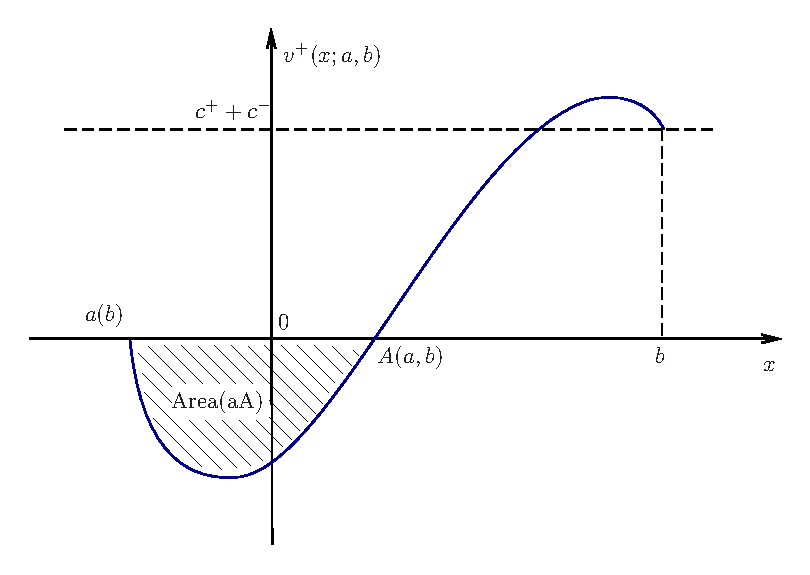
\includegraphics[scale=0.6]{a}
\end{figure}

\proof{Proof}{It can be shown.\\
The next line\Halmos}

\endproof
\begin{lemma}
We find
\end{lemma}


\proof{Proof}{Deferred\Halmos}

\endproof
\begin{proposition}
We find
\end{proposition}


\proof{Proof}{Deferred\Halmos}

\endproof

\subsubsection*{Algorithm. }
\begin{enumerate}
\item Computation: 

\begin{enumerate}
\item Compute: 

\begin{enumerate}
\item Solve; 
\end{enumerate}
\end{enumerate}
\end{enumerate}

\subsection{Tests}

In this sub-section 

\begin{table}[H]
\caption{\label{tab:Numerical-comparison-without-SAGC}Numerical}
\centering{}%
\begin{tabular}{|c|c|>{\centering}p{2cm}|c|}
\hline 
Case & algorithm & time

(millisecond) & iterations\tabularnewline
\hline 
\hline 
0 & B & 0.197 & 3\tabularnewline
\cline{2-4} 
 & F & 2940 & 7\tabularnewline
\hline 
\end{tabular}
\end{table}

\textbf{Model:}

$a=0,q=0.56$;

It \citep{alvarez2008optimal} has been proved by \citealt{alvarez2008optimal}.

\theendnotes
\begin{thebibliography}{{Alvarez(2008)}}
\bibitem[{Alvarez(2008)}]{alvarez2008optimal}Alvarez, L.H.R., J.
Lempa. 2008. On the optimal. \textit{SIAM Journal}, 47:703.
\end{thebibliography}

\ECSwitch \ECHead{Companion Document Title}

\section{Introduction}
\begin{repeattheorem}[Theorem \ref{thm:thm1}.]
 aaa
\end{repeattheorem}


\subsection{Formulation\label{subsec:Formulation-of-the-1}}
\begin{repeattheorem}[Theorem 2.]
asdfasdf
\end{repeattheorem}


\end{document}
